\RequirePackage{ifpdf}

\documentclass[a4paper,12pt]{article}
\ifpdf
  \usepackage[pdftex]{graphicx}
\else
  \usepackage[dvips]{graphicx}
\fi
\usepackage{epsfig}
\usepackage{rotating}
\usepackage{listings}
\usepackage{booktabs}
\usepackage{fancyhdr}
\usepackage{float}
\floatplacement{figure}{H}
\floatplacement{table}{H}



\begin{document}


\section{Accuracy of local coordinate measurement}


\begin{figure}[t]
%\centering
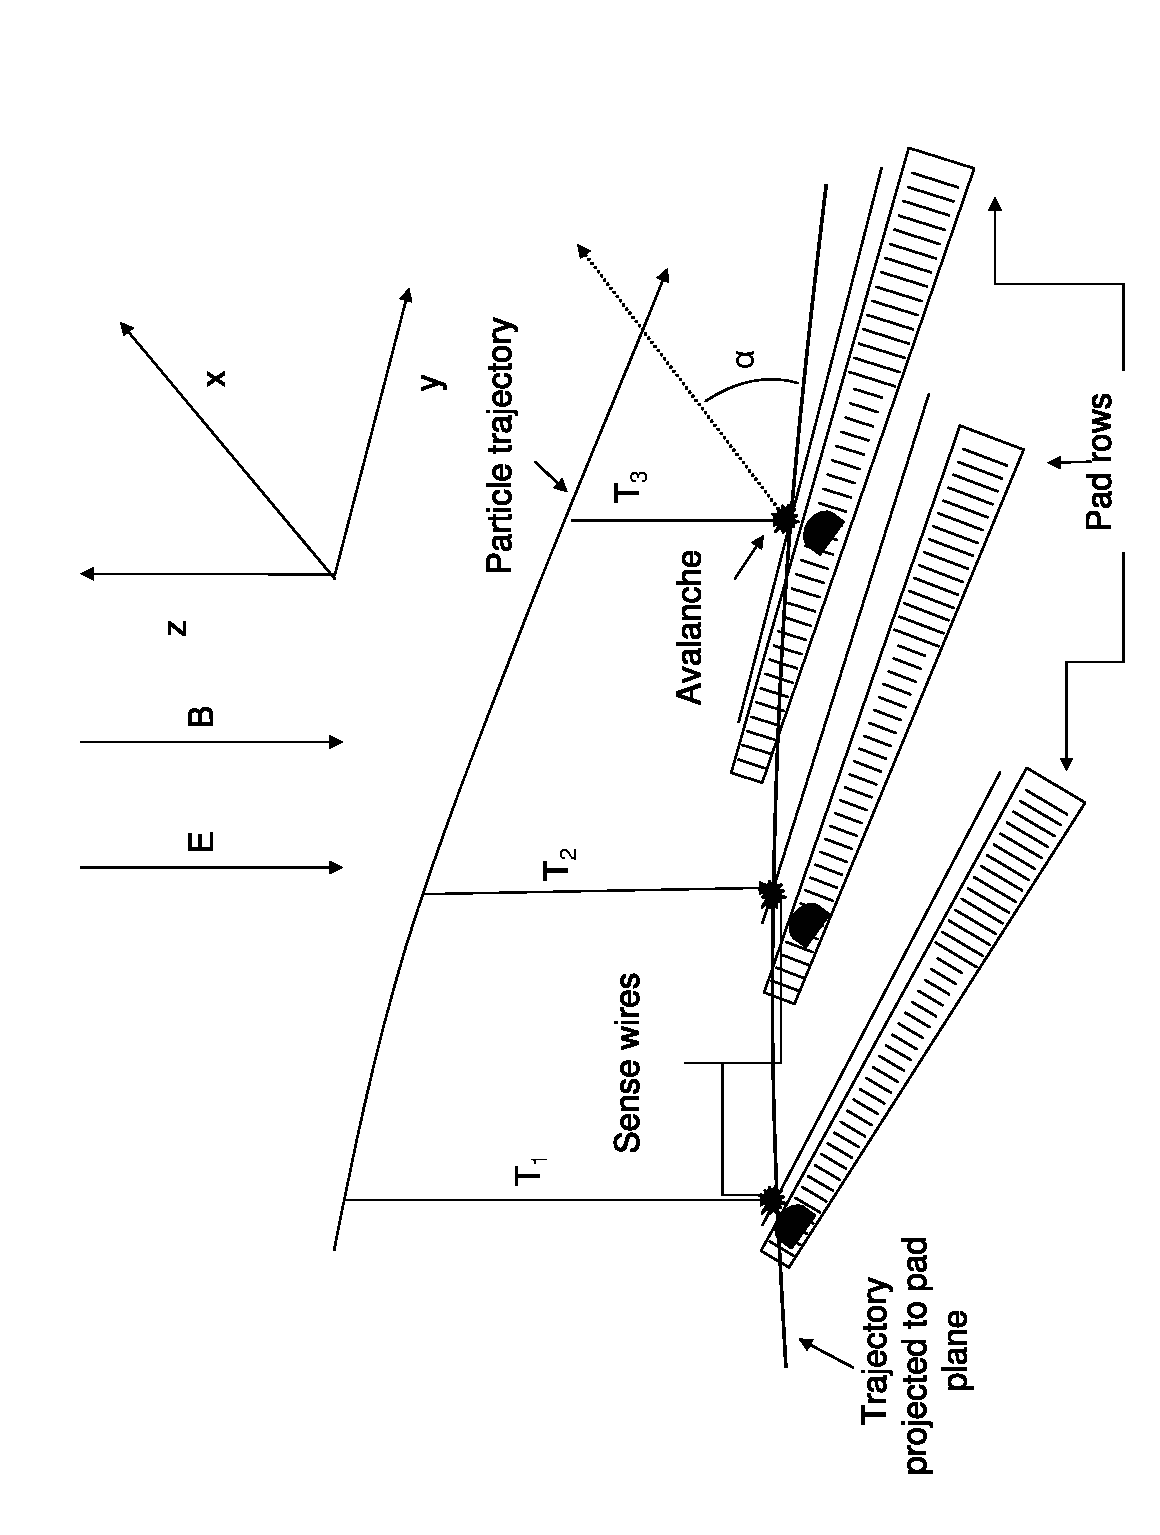
\includegraphics[width=60mm,angle=-90]{picCluster/pic2.eps}
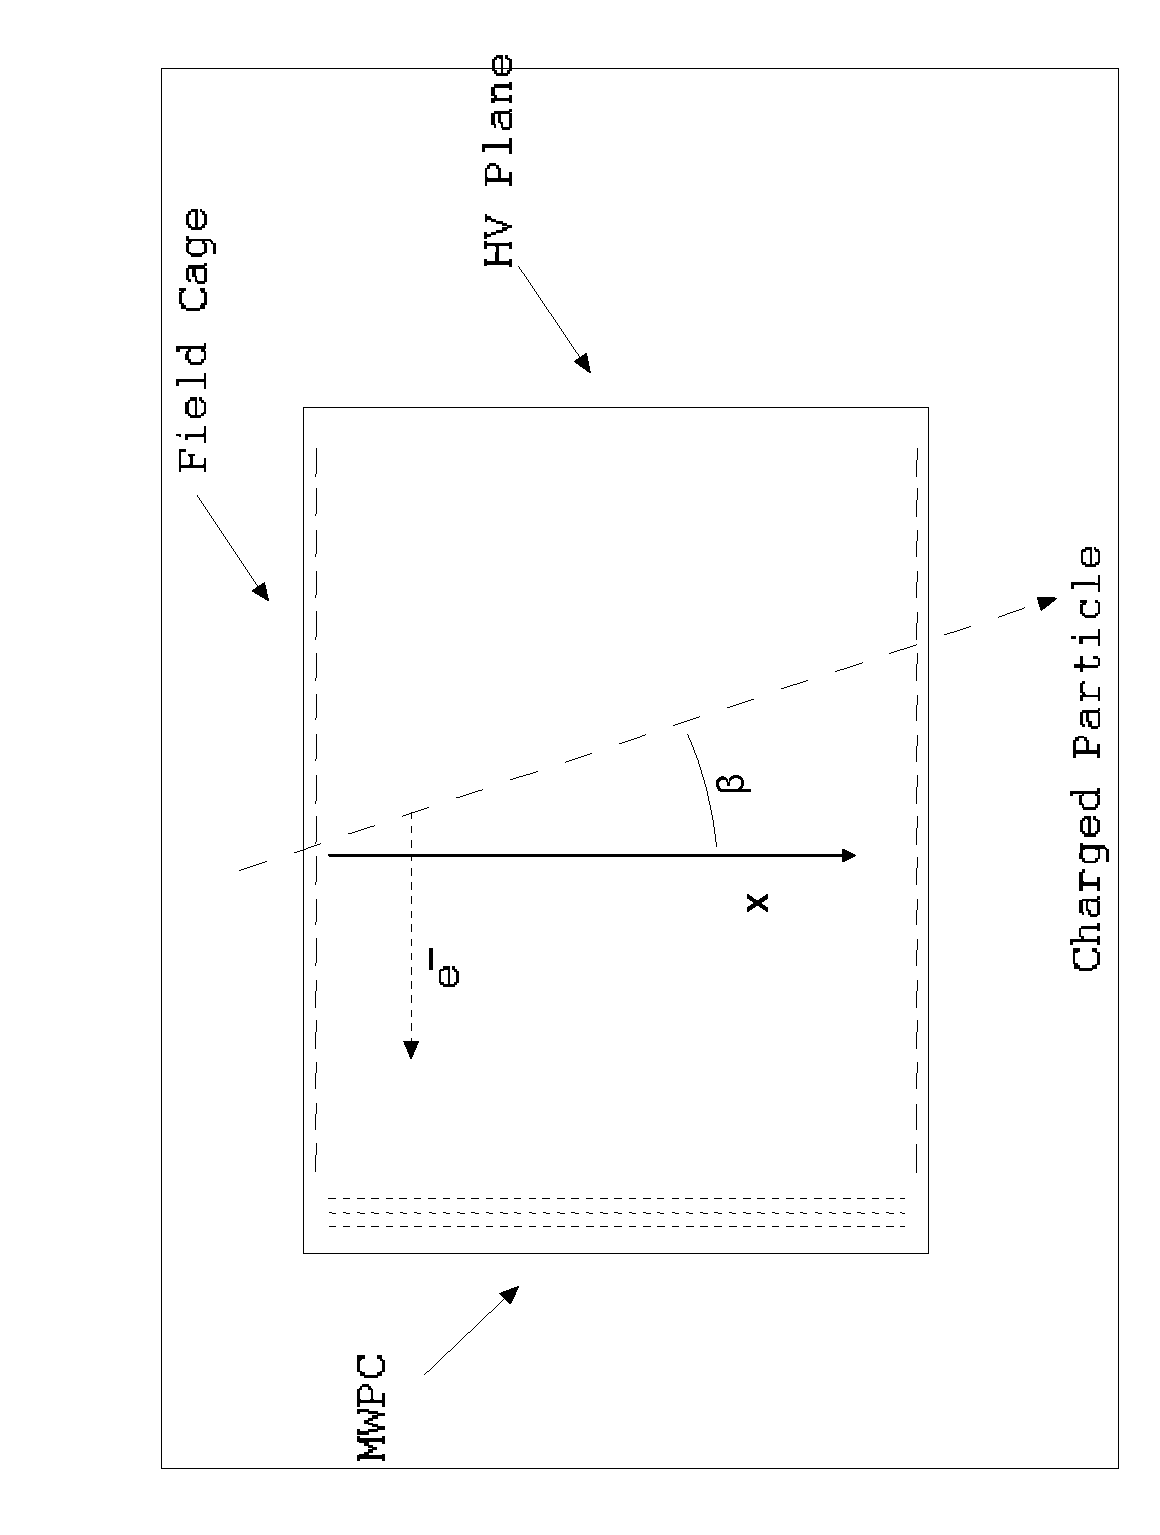
\includegraphics[width=60mm,angle=-90]{picCluster/pic1.eps}
\caption{Schematic view of the detection process in TPC  (upper
part - perspective view, lower part - side view).} \label{figTPC}
\end{figure}

The accuracy of the coordinate measurement is limited by a track
angle which spreads ionization and by diffusion which amplifies
this spread.

The track direction with respect to pad plane is given by two
angles $\alpha$ and $\beta$ (see fig.~\ref{figTPC}). For the
measurement along the pad-row, the angle $\alpha$ between the
track projected onto the pad plane and pad-row is relevant. For
the measurement of the the drift coordinate ({\it{z}}--direction)
it is the angle $\beta$ between the track and {\it{z}} axis
(fig.~\ref{figTPC}).

The ionization electrons are randomly distributed along the
particle trajectory. Fixing the reference {\it{x}} position of an
electron at the middle of pad-row, the {\it{y}} (resp. {\it{z}})
position of the electron is a random variable characterized by
uniform distribution with the width $L_{\rm{a}}$, where
$L_{\rm{a}}$ is given by the pad length $L_{\rm{pad}}$ and the
angle $\alpha$ (resp. $\beta$):
\[L_{\rm{a}}=L_{\rm{pad}}\tan\alpha\]

The diffusion smears out the position of the electron with
gaussian probability distribution with $\sigma_{\rm{D}}$.
Contribution of the $\mathbf{E{\times}B}$ and unisochronity
effects for the  Alice TPC are negligible. The typical resolution
in the case of ALICE TPC is on the level of
$\sigma_{y}\sim$~0.8~mm and $\sigma_{z}\sim$~1.0~mm integrating
over all clusters in the TPC.



\subsection{Gas gain fluctuation effect}

Being collected on sense wire, electron is "multiplied" in strong
electric field. This multiplication is subject of a large
fluctuations, contributing to the cluster position resolution.
Because of these fluctuations the center of gravity of the
electron cloud can be shifted.

Each electron is amplified independently. However, in the
reconstruction electrons are not treated separately. The Centre Of
Gravity  (COG) of the cluster is usually used as an estimation for
the local track position. The influence of the gas gain
fluctuation to the reconstructed point characteristic can be
described by a simple model, introducing a weighted COG
$X_{\rm{COG}}$
\begin{eqnarray}
    X_{\rm{COG}}=\frac{\sum_{i=1}^{N}{g_ix_i}}{\sum_{i=1}^N{g_i}},
\label{eqCOGdefGG}
\end{eqnarray}
where {\it{N}} is the total number of electrons in the cluster and
$g_i$ is a random variable equal to a gas amplification for given
electron.

The mean value of $X_{\rm{COG}}$ is equal to the mean value
$\overline{x}$ of the original distribution of electrons
\begin{eqnarray}
      \overline{X_{COG}}=
    \overline{\frac{\sum_{i=1}^{N}{g_ix_i}}{\sum_{i=1}^N{g_i}}}
    =\overline{x}\overline{\frac{\sum_{i=1}^{N}{g_i}}
    {\sum_{i=1}^N{g_i}}} =\overline{x}.
\label{eqCOGMeanGG}
\end{eqnarray}

However, the same is not true for the dispersion of the position,
%$\sigma^2_{X_{COG}}\sigma_x^2$:
%\begin {center}
\begin{eqnarray}
    \lefteqn{ \sigma^2_{X_{\rm{COG}}}
    =\overline{X_{\rm{COG}}^2}-\overline{X_{\rm{COG}}}^2=}\nonumber\\&&{}
    =\overline{\left(\frac{1}{\sum_{i=1}^N{g_i}}\sum_{i=1}^{N}{g_ix_i}
    \right)^2}-\overline{x}^2=
    \nonumber\\
    &&{}=\overline{\frac{{\sum\sum{x_ix_jg_ig_j}}}{{\sum\sum{g_ig_j}}}}-
    \overline{x}^2=
    \nonumber\\&&{}=
    \overline{x^2}\overline{\frac{\sum_i{g_i^2}}{\sum\sum{g_ig_j}}}-
    \overline{x}^2
    \overline{\frac{\sum\sum{g_ig_j}-\sum\sum_{i\ne{j}}{g_ig_j}}
    {\sum\sum{g_ig_j}}}= \nonumber\\&&
    =\left(\overline{x^2}-\overline{x}^2\right)
    \overline{\frac{\sum{g_i^2}}{\sum\sum{g_ig_j}}}=
    \sigma_x^2\overline{\frac{\sum{g_i^2}}{\sum\sum{g_ig_j}}}=
    \nonumber\\
    &&{}=\frac{\sigma_x^2}{N}{\times}G_{\rm{gfactor}}^2
\label{eqCOGSigmaGG}
\end{eqnarray}

where
\begin{eqnarray}
      G_{\rm{gfactor}}^2 = N\overline{\frac{\sum{g_i^2}}{\sum\sum{g_ig_j}}}
\label{eqCOGGGfactor0}
\end{eqnarray}

The diffusion term is effectively multiplied by gas gain factor
$G_{\rm{gfactor}}$. For sufficiently large number of electrons,
when $g_i^2$ and $\sum\sum{g_ig_j}$ are quasi independent
variables, equation (\ref{eqCOGGGfactor0}) can be transformed to
the following

\begin{eqnarray}
    \lefteqn{G_{\rm{gfactor}}^2 \approx
    N\frac{\overline{\sum{g_i^2}}}
    {\overline{\sum\sum{g_ig_j}}}}\nonumber\\
    &&{} =
    N\frac{N\overline{g^2}}{N(N-1)\overline{g}^2+N\overline{g^2}}=
    \nonumber\\
    &&{} =N\frac{ \left(\sigma_g^2/\overline{g}^2+1 \right)}
    {N+\sigma_g^2/\overline{g}^2}
\label{eqCOGGGfactorE}
\end{eqnarray}

Gas gain fluctuation of the gas detector working in proportional
regime is described with the exponential distribution with the
mean value $\bar{g}$ and r.m.s.
\begin{eqnarray}
        \sigma_{\rm{g}} =\bar{g}
\label{eqSigmaexp}
\end{eqnarray}

Substituting $\sigma_{\rm{g}}$ into equation
(\ref{eqCOGGGfactorE})
\begin{eqnarray}
    G_{\rm{gfactor}}^2 =\frac{2N}{N+1}.
\label{eqCOGGGfactorR}
\end{eqnarray}

Gas multiplication fluctuation in chamber  deteriorates
$\sigma_{X_{\rm{COG}}}$  by a factor of about ${\sqrt{2}}$. The
prediction of this model is in good agreement with results from
the simulation.


\subsection{Secondary ionization effect}

Charged particle penetrating the gas of the detector produces
{\it{N}} primary electrons. Primary electron {\it{i}} produces
$n_{\rm{s}}^i-1$ secondary electrons. Each of these electrons is
amplified in the electric field by a factor of $g_j$.

Each primary cluster is characterized by a position $x_i$ with
mean value $\overline{x}$ and $\sigma_x$. The COG given by
equation (\ref{eqCOGdefGG}) is modified to the following form:

\begin{eqnarray}
    X_{\rm{COG}}=\frac{1}{\sum_{i=1}^N\sum_{j=1}^{n_i}{g_j^{i}}}
    \sum_{i=1}^{N}{x_i}\sum_{j=1}^{n_i}{g_j^{i}}.
\label{eqCOGdefGGPIO}
\end{eqnarray}
A new variable $G_n$ is introduced as the total electron gain:
\begin{eqnarray}
    G_n=\sum_{j=1}^{n}{g_j}.
\label{eqGNdef}
\end{eqnarray}


Knowing the distribution of {\it{n}} and {\it{g}} and assuming
that {\it{n}} and {\it{g}} are independent variables  the mean
value and variance of the $G_n$ can be expressed as:

\begin{eqnarray}
    \lefteqn{
    \overline{G_n}=\overline{n}\overline{g}} \\
    &&{}
    \frac{\sigma^2_{G_n}}{\overline{G_n^2}}=
    \frac{\sigma^2_n}{\overline{n}^2}+
    \frac{\sigma^2_g}{\overline{g}^2}
    \frac{1}{\overline{n}}
\label{eqGNsigma}
\end{eqnarray}

Inserting $G_n$ into equation (\ref{eqCOGdefGGPIO}) results in an
equation similar to the equation (\ref{eqCOGdefGG}).

Multiplicative factor $G_{\rm{Lfactor}}$ is defined as an analog
of $G_{\rm{gfactor}}$, from the equation (\ref{eqCOGGGfactor0})
\begin{eqnarray}
    G_{\rm{Lfactor}}^2 =  N\frac{\overline{\sum{G_i^2}}}
    {\overline{\sum\sum{G_iG_j}}}.
\label{eqCOGLfactor0}
\end{eqnarray}

Using the new variable $G_n$ and simply replacing  gas gain
{\it{g}} by $G_n$ in the similar way as in equation
(\ref{eqCOGGGfactorE}) does not work. For $1/E^{2}$
parametrization of secondary ionization process
$\sigma^2_{G_n}/\overline{G_n}$ goes to infinity and thus
$\sigma^2_{X_{COG}}=\sigma_x^2$. Moreover $G_i^2$ and
$\sum\sum{G_iG_j}$ are not quasi independent as the sum
$\sum\sum{G_iG_j}$ could be given by one "exotic" electron
cluster. Approximations used for deriving the equation
(\ref{eqCOGGGfactorE}) are not valid for secondary ionization
effect.

In order to estimate the impact of this effect on COG  equation
(\ref{eqCOGLfactor0}) has to be solved numerically. Simulation
showed that $G_{\rm{Lfactor}}$ does not depend strongly on the cut
used for maximum number of electrons created in the process of
secondary ionization. A change of the cut,  from 1000 electrons up
produces a change of about 3\% in $G_{\rm{Lfactor}}$.

Equation (\ref{eqCOGGGfactorE}) is not applicable in this
situation because of the infinity of the $\sigma_G$. According to
the simulation, the threshold  on the number of electrons in the
cluster  has a little influence to the resulting
$G_{\rm{Lfactor}}$. Therefore we fit simulated $G_{\rm{Lfactor}}$
with formula (\ref{eqCOGGGfactorE}) where
$\sigma_G^2/\overline{G}^2$ was a free parameter. However, this
parametrization does not describe the data for wide enough range
of {\it{N}}. In further study the linear parametrization of the
COG factor was used. This parametrization was validated on
reasonable interval of {\it{N}}.



\section{Center-of-gravity error parametrization}

Detected position of charged particle  is a random variable given
by several stochastic processes: diffusion, angular effect, gas
gain fluctuation, Landau fluctuation of the secondary ionization,
$\mathbf{E{\times}B}$ effect, electronic noise and systematic
effects (like space charge, etc.). The relative influence of these
processes to the resulting distortion of position determination
depends on the detector parameters. In the big drift detectors
like the ALICE TPC the main contribution is given by diffusion,
gas gain fluctuation, angular effect and secondary ionization
fluctuation.

Furthermore we will use following  assumptions:
\begin{itemize}
\item $N_{\rm{prim}}$ primary electrons  are produced at a random
positions $x_i$ along the particle trajectory. \item $n_i-1$
electrons are produced in the process of secondary ionization.
\item Displacement of produced electrons due to the thermalization
is neglected.
\end{itemize}

Each of electrons is characterized by a random vector
$\vec{z}^i_j$
\begin{eqnarray}
    \vec{z}^i_j =\vec{x}^i+\vec{y}^i_j,
\label{eqZtot}
\end{eqnarray}
where {\it{i}} is the index of primary electron cluster and
{\it{j}} is the index of the secondary electron inside of the
primary electron cluster. Random variable $\vec{x}^i$ is a
position where the primary electron was created. The position
$\vec{y}^i_j$ is a random variable specific for each electron.  It
is given mainly by a diffusion.

The center of gravity of the electron  cloud is given:
\begin{eqnarray}
    \lefteqn{\vec{z}_{\rm{COG}}=\frac{1}{\sum_{i=1}^{N_{\rm{prim}}}
    \sum_{j=1}^{n_i}{g_j^i}}
    \sum_{i=1}^{N_{\rm{prim}}}\sum_{j=1}^{n_i}{g_j^i\vec{z}_j^i}=}
    \nonumber\\
    &&{}\frac{1}{\sum_{i=1}^{N_{\rm{prim}}}
    \sum_{j=1}^{n_i}{g_j^i}}
    \sum_{i=1}^{N_{\rm{prim}}}\vec{x}^i\sum_{j=1}^{n_i}{g_j^i}+\nonumber\\
    &&{}\frac{1}{\sum_{i=1}^{N_{\rm{prim}}}
    \sum_{j=1}^{n_i}{g_j^i}}
    \sum_{i=1}^{N_{\rm{prim}}}\sum_{j=1}^{n_i}{g_j^i\vec{y}_j^i}=
    \nonumber\\ \nonumber\\
    &&{}
    \vec{x}_{\rm{COG}}+\vec{y}_{\rm{COG}}.
\label{eqCOGSec}
\end{eqnarray}

The mean value $\overline{\vec{z}_{\rm{COG}}}$ is equal to the sum
of mean values $\overline{\vec{x}_{\rm{COG}}}$ and
$\overline{\vec{y}_{\rm{COG}}}$.

The sigma of COG in one of the dimension of vector
$\vec{z}_{1COG}$ is given by following equation
\begin{eqnarray}
    \lefteqn{\sigma_{z_{\rm{1COG}}}^2=\sigma_{x_{\rm{1COG}}}^2+
    \sigma_{y_{\rm{1COG}}}^2+}\nonumber\\
    &&{}
        2\left(\overline{x_{\rm{1COG}}y_{\rm{1COG}}}-\bar{x}_{\rm{1COG}}
        \bar{y}_{1COG}\right).
\label{eqCOGSigSec}
\end{eqnarray}

If the vectors $\vec{x}$ and $\vec{y}$ are independent random
variables the last term in the equation (\ref{eqCOGSigSec}) is
equal to zero.
\begin{eqnarray}
    \sigma_{z_{1COG}}^2=\sigma_{x_{\rm{1COG}}}^2+
    \sigma_{y_{\rm{1COG}}}^2,
\label{eqCOGSigSecIn}
\end{eqnarray}
r.m.s. of COG distribution is given by the sum of r.m.s of
{\it{x}} and {\it{y}} components.

In order to estimate the influence of the $\mathbf{E{\times}B}$
and unisochronity effect to the space resolution  two additional
random vectors are added to the initial electron position.


\begin{eqnarray}
\vec{z}^i_j =\vec{x}^i+\vec{y}^i_j+
        \vec{X}_{\mathbf{E{\times}B}}(\vec{x}^i+\vec{y}^i_j)+
        \vec{X}_{\rm{Unisochron}}(\vec{x}^i+\vec{y}^i_j).
\label{eqZtotplus}
\end{eqnarray}
The probability distributions of $\vec{X}_{\mathbf{E{\times}B}}$
and $\vec{X}_{\rm{Unisochron}}$ are  functions of  random vectors
$\vec{x^i}$ and $\vec{y^i_j}$, and they are strongly correlated.
However, simulation indicates that in large drift detectors
distortions, due to these effects,  are negligible compared with a
previous one.

Combining previous equation and neglecting $\mathbf{E{\times}B}$
and unisochronity
effects, the COG distortion  parametrization appears as:\\
{$\sigma_{z}$} of cluster center in {\it{z}} (time) direction
\begin{eqnarray}\
     \lefteqn{\sigma^2_{{z_{\rm{COG}}}} = \frac{D^2_{\rm{L}}
     L_{\rm{Drift}}}{N_{\rm{ch}}}G_{\rm{g}}+}\nonumber\\&&{}
        \frac{{\tan^2\alpha}~L_{\rm{pad}}^2G_{\rm{Lfactor}}(N_{\rm{chprim}})}{12N_{\rm{chprim}}}+
        \sigma^2_{\rm{noise}},
         \label{eqResZ1}
\end{eqnarray}

and {$\sigma_{y}$} of cluster center in {\it{y}}(pad) direction
    \begin{eqnarray}
     \lefteqn{\sigma^2_{y_{\rm{COG}}} = \frac{D^2_{\rm{T}}L_{\rm{Drift}}}{N_{\rm{ch}}}G_{\rm{g}}+}\nonumber\\&&{}
        \frac{{\tan^2\beta}~L_{\rm{pad}}^2G_{\rm{Lfactor}}(N_{\rm{chprim}})}{12N_{\rm{chprim}}}+
        \sigma^2_{\rm{noise}},
        \label{eqResY1}
    \end{eqnarray}
 where
${N_{\rm{ch}}}$ is the total number of electrons in the cluster,
${N_{\rm{chprim}}}$ is the number of primary electrons in the
cluster, ${G_{\rm{g}}}$ is the gas gain fluctuation factor,
${G_{\rm{Lfactor}}}$ is the secondary ionization fluctuation
factor and $\sigma_{\rm{noise}}$ describe the contribution of the
electronic noise to the resulting sigma of the COG.

\section{Precision of cluster COG determination using measured
amplitude}

We have derived parametrization using as parameters the total
number of electrons ${N_{\rm{ch}}}$ and the number of primary
electrons ${N_{\rm{chprim}}}$. This parametrization is in good
agreement with simulated data, where the ${N_{\rm{ch}}}$ and
${N_{\rm{chprim}}}$ are known. It can be  used as an estimate for
the limits of accuracy, if the mean values
$\overline{N}_{\rm{ch}}$ and $\overline{N}_{\rm{chprim}}$ are used
instead.

The ${N_{\rm{ch}}}$ and ${N_{\rm{chprim}}}$ are random variables
described by a Landau distribution, and  Poisson distribution
respectively .

In order to use previously derived formulas (\ref{eqResZ1},
\ref{eqResY1}), the number of electrons can be estimated  assuming
their proportionality to the total measured charge $A$ in the
cluster. However, it turns out that an empirical parametrization
of the factors $G(N)/N=G(A)/(kA)$ gives better results.
Formulas (\ref{eqResZ1}) and (\ref{eqResY1}) are transformed to following form:\\

{$\sigma_{z}$} of cluster center in {\it{z}} (time) direction:
    \begin{eqnarray}
     \lefteqn{\sigma^2_{z_{\rm{COG}}} =
     \frac{D^2_{\rm{L}}L_{\rm{Drift}}}{A}{\times}\frac{G_g(A)}{k_{\rm{ch}}}+}\nonumber\\
        &&{}
        \frac{\tan^2\alpha~L_{\rm{pad}}^2}{12A}{\times}\frac{G_{Lfactor}(A)}{k_{\rm{prim}}}+\sigma^2_{\rm{noise}}
        \label{eqZtotAmp}
    \end{eqnarray}

and {$\sigma_{y}$} of cluster center in {\it{y}}(pad) direction:
    \begin{eqnarray}
     \lefteqn{\sigma_{y_{\rm{COG}}} =
     \frac{D^2_{\rm{T}}L_{\rm{Drift}}}{A}{\times}\frac{G_g(A)}{k_{\rm{ch}}}+}\nonumber\\
        &&{}
        \frac{\tan^2\beta~L_{\rm{pad}}^2}{12A}{\times}\frac{G_{Lfactor}(A)}{k_{\rm{prim}}}+\sigma^2_{\rm{noise}}
        \label{eqYtotAmp}
    \end{eqnarray}

\section{Estimation of the precision of cluster  position
determination using measured cluster shape}

The shape of the cluster is given by the convolution of the
responses to the electron avalanches. The time response function
and the pad response function are almost gaussian, as well as the
spread of electrons due to the diffusion. The spread due to the
angular effect is uniform. Assuming that the contribution of the
angular spread does not dominate the cluster width, the cluster
shape is not far from gaussian. Therefore, we can use the
parametrization

\begin{equation}
       f(t,p) = K_{\rm{Max}}.\exp\left(-\frac{(t-t_{\rm{0}})^2}{2\sigma_{\rm{t}}^2}-
            \frac{(p-p_{\rm{0}})^2}{2\sigma_{\rm{p}}^2}\right),
            \label{eq:GaussTP}
\end{equation}
where  ${K_{\rm{Max}}}$ is the  normalization factor, $t$ and $p$
are time and pad bins, $t_0$ and $p_0$ are centers of the cluster
in time and pad direction and $\sigma_{\rm{t}}$ and
$\sigma_{\rm{p}}$ are the r.m.s. of the time and pad cluster
distribution.

 The mean width of the cluster distribution is given by:
\begin{equation}
     \sigma_{\rm{t}} = \sqrt{D{\rm{^2_L}}L_{\rm{drift}}+\sigma^2_{\rm{preamp}}+
        \frac{\tan^2\alpha~L_{\rm{pad}}^2}{12}},
\end{equation}


\begin{equation}
     \sigma_{\rm{p}} = \sqrt{D{\rm{^2_T}}L_{\rm{drift}}+\sigma^2_{\rm{PRF}}+
        \frac{\tan^2\beta~L_{\rm{pad}}^2}{12}},
\end{equation}
where ${\sigma_{\rm{preamp}}}$ and ${\sigma_{\rm{PRF}}}$  are the
r.m.s. of the time response function and  pad response function,
respectively.

The fluctuation of the shape depends on the contribution of the
random diffusion and angular spread, and on the contribution given
by a gas gain fluctuation and secondary ionization. The
fluctuation of the time and pad response functions is small
compared with the previous one.

The measured r.m.s of the cluster is influenced by a threshold
effect.
\begin{equation}
     \sigma_{\rm{t}}^2 = \sum_{A(t,p)>\rm{threshold}}{(t-t_{\rm{0}})^2{\times}A(t,p)}
\end{equation}
The threshold effect can be eliminated using two dimensional
gaussian fit instead of the simple COG method. However, this
approach is slow and, moreover, the result is very sensitive to
the gain fluctuation.

To eliminate the threshold effect in r.m.s. method, the bins
bellow threshold are replaced with a virtual charge  using
gaussian interpolation of the cluster shape. The introduction of
the virtual charge improves the precision of the COG measurement.
Large systematic shifts in the estimate of the cluster position
(depending on the local track position relative to pad--time) due
to the threshold are no longer observed.

Measuring the r.m.s. of the cluster, the local diffusion and
angular spread of the electron cloud can be estimated. This
provides  additional information for the estimation of
distortions. A simple additional correction function is used:
\begin{eqnarray}
     \sigma_{\rm{COG}} \rightarrow
     \sigma_{\rm{COG}}(A){\times}(1+{\rm{const} {\times}\frac{\delta
     \rm{RMS}}{\rm{teorRMS}}}),
\label{eqResUsingRMS}
\end{eqnarray}
where $\sigma_{\rm{COG}}(A)$ is calculated according formulas
\ref{eqResY1} and \ref{eqResZ1}, and the
$\delta\rm{RMS}/\rm{teorRMS}$ is the relative distortion of the
signal shape from the expected one.






\section{TPC cluster finder}

The classical approach for the beginning of the tracking was
chosen. Before the tracking itself, two-dimensional clusters in
pad-row--time planes are found. Then the positions of the
corresponding space points are reconstructed, which are
interpreted as the crossing points of the tracks and the centers
of the pad rows. We investigate the region 5$\times$5 bins in
pad-row--time plane around the central bin with maximum amplitude.
The size of region, 5$\times$5 bins, is bigger than typical size
of cluster as the $\sigma_{\rm{t}}$ and $\sigma_{\rm{pad}}$ are
about 0.75 bins.

The COG and r.m.s are used to characterize cluster. The COG and
r.m.s are affected by systematic distortions induced by the
threshold effect. Depending on the number of time bins and pads in
clusters the COG and r.m.s. are affected in different ways.
Unfortunately, the number of bins in cluster is the function of
local track position. To get rid of this effect, two-dimensional
gaussian fitting can be used.

Similar results can be achieved  by so called r.m.s. fitting using
virtual charge. The signal below threshold is replaced by the
virtual charge, its expected value according a interpolation. If
the virtual charge is above the threshold value, then it is
replaced with amplitude equal to the threshold value. The signal
r.m.s is used for later error estimation  and as a criteria for
cluster unfolding. This method gives comparable results as
gaussian fit of the cluster but is much faster. Moreover, the COG
position is less sensitive to the gain fluctuations.

The cluster shape depends on the track parameters.  The response
function contribution and diffusion contribution to the cluster
r.m.s. are known during clustering. This is not true for a angular
contribution to the cluster width. The cluster finder should be
optimised for high momentum particle coming from the primary
vertex. Therefore, a conservative approach was chosen, assuming
angle $\alpha$ to be zero. The tangent of the angle $\beta$ is
given by  {\it{z}}-position and pad-row radius, which is known
during clustering.


\subsection{Cluster unfolding}

The estimated width of the cluster is used as criteria for cluster
unfolding. If the r.m.s. in one of the directions is greater then
critical r.m.s,  cluster is considered for unfolding. The fast
spline method is used here. We require the charge to be conserved
in this method. Overlapped clusters  are supposed to have the same
r.m.s., which is equivalent to the same track angles. If this
assumption is not fulfilled, tracks diverge very rapidly.


\begin{figure}[t]
\centering
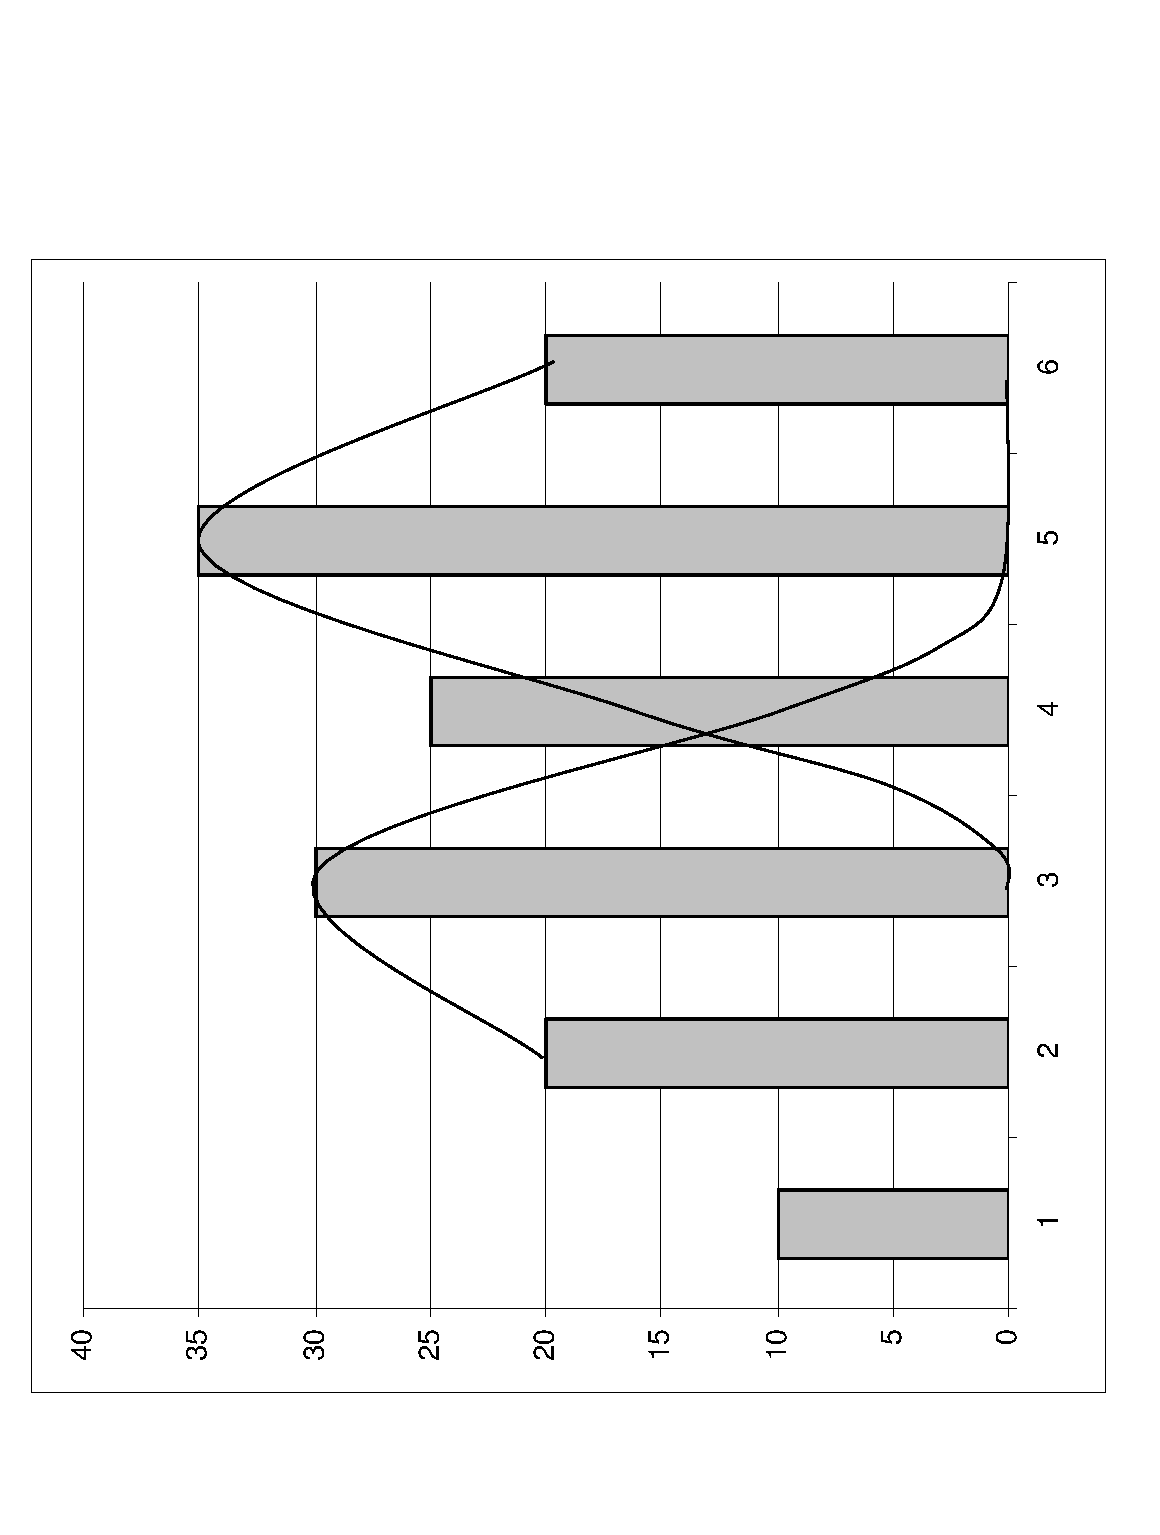
\includegraphics[width=60mm,angle=-90]{picCluster/unfolding1.eps}
\caption{
Schematic view of unfolding principle.} \label{figUnfolding1}
\end{figure}
\begin{figure}[t]
\centering
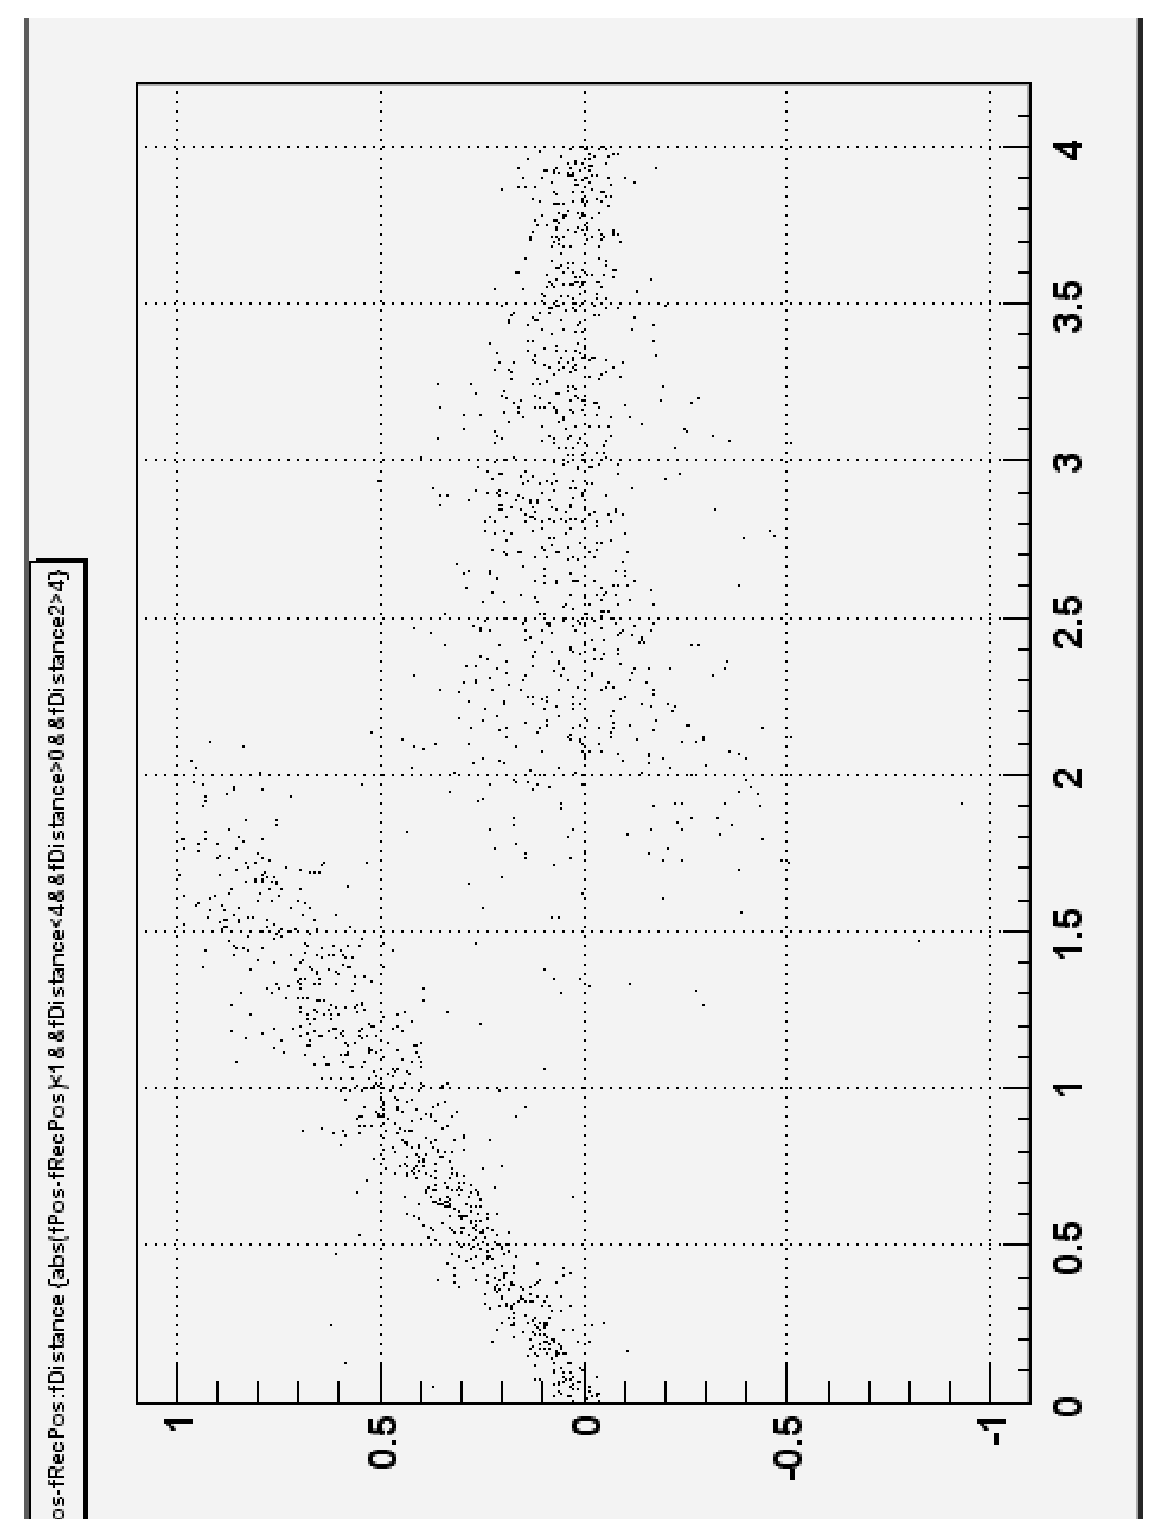
\includegraphics[width=60mm,angle=-90]{picCluster/unfoldingres.eps}
\caption{ Dependence of the position residual as function of the
distance to the second cluster.} \label{figUnfoldingRes}
\end{figure}

The unfolding algorithm has the following steps:
\begin{itemize}

\item Six amplitudes $C_i$ are investigated (see fig.
\ref{figUnfolding1}). First (left) local maxima, corresponding to
the first cluster is placed at position 3, second (right) local
maxima corresponding to the second cluster is at position 5.

\item In the first iteration, amplitude in bin 4 corresponding to
the cluster on left side $A_{\rm{L4}}$ is calculated using
polynomial interpolation, assuming virtual amplitude at
$A_{\rm{L5}}$ and derivation at $A_{\rm{L5}}^{'}$ to be 0.
Amplitudes $A_{\rm{L2}}$ and $A_{\rm{L3}}$ are considered to be
not influenced by overlap ($A_{\rm{L2}}=C_2$ and
$A_{\rm{L3}}=C_3)$.

\item The amplitude $A_{\rm{R4}}$ is calculated in similar way. In
the next iteration the amplitude $A_{\rm{L4}}$ is calculated
requiring charge conservation
$C_{\rm{4}}=A_{\rm{R4}}+A_{\rm{L4}}$. Consequently
\begin{eqnarray}
   A_{\rm{L4}} \rightarrow
   C_{\rm{4}}\frac{A_{\rm{L4}}}{A_{\rm{L4}}+A_{\rm{R4}}}
\end{eqnarray}
and
\begin{eqnarray}
   A_{\rm{R4}} \rightarrow
   C_{\rm{4}}\frac{A_{\rm{R4}}}{A_{\rm{L4}}+A_{\rm{R4}}}.
\end{eqnarray}
\end{itemize}


Two cluster resolution depends on the distance between the two
tracks. Until  the shape of cluster triggers unfolding, there is a
systematic shifts towards to the COG of two tracks (see fig.
\ref{figUnfoldingRes}), only one cluster is reconstructed.
Afterwards, no systematic shift is observed.


\subsection{Cluster characteristics}

The cluster is characterized by the COG in {\it{y}} and {\it{z}}
directions (fY and fZ) and  by the cluster width (fSigmaY,
fSigmaZ). The deposited charge is described by the signal at
maximum (fMax), and total charge in cluster (fQ). The cluster type
is characterized by the data member fCType which is defined as a
ratio of the charge supposed to be deposited by the track and
total charge in cluster in investigated region 5$\times$5. The
error of the cluster position is assigned to the cluster only
during tracking according formulas
 (\ref{eqZtotAmp}) and  (\ref{eqYtotAmp}), when track
 angles $\alpha$ and $\beta$ are known with sufficient precision.


Obviously, measuring the position of each electron separately the
effect of the gas gain fluctuation can be removed, however this is
not easy to implement in the large TPC detectors. Additional
information about cluster asymmetry can be used, but the resulting
improvement of around 5\% in precision on simulated data  is
negligible, and it is questionable, how successful will be such
correction for the cluster asymmetry on real data.

However, a cluster asymmetry can be used as additional  criteria
for cluster unfolding. Let's denote $\mu_i$ the {\it{i}}-th
central momentum of the cluster, which was created by overlapping
from two sub-clusters with unknown positions and deposited energy
(with momenta $^1\mu_i$ and $^2\mu_i$).

Let $r_1$ is the ratio of two clusters amplitudes:
\[r_1={^1\mu_0}/({^1\mu_0}+{^2\mu_0})\] and the track  distance {\it{d}} is equal to
\[d = {^1\mu_1} -{^2\mu_1}.\]

Assuming that the second moments for both sub-clusters are the
same (${^0\mu_2}={^1\mu_2}={^2\mu_2}$), two sub-clusters distance
{\it{d}} and amplitude ratio $r_1$ can be estimated:
\begin{eqnarray}
     R   = \frac{(\mu_3^6)}{(\mu_2^2-{^0\mu_2^2})^3}\\
    r_{\rm{1}} =0.5\pm0.5{\times}\sqrt{\frac{1}{1-4/R}}  \\
    d   = \sqrt{(4+R){\times}(\mu_2^2-{^0\mu_2^2})}
\label{eqMeas}
\end{eqnarray}

In order to trigger unfolding using the shape information
additional  information about track and mean cluster shape over
several pad-rows are needed. This information is available only
during tracking procedure.



\subsection{Space point resolution parameterization}

The space point resolution is the function of many parameters but for the ALICE TPC the dominant one are the diffusion, track inclination angle and deposited charge.
The space point resolution was extracted from the data in bins of these variables.

In the first approximation the angular part and diffusion part are independent. The
paramaterization is obtained fitting parameters $p_{0}$,$p_L$ and $p_A$
\begin{eqnarray}\
     \sigma^2_{{\rm{COG}}} \approx p^2_0+p^2_{L}L_{\rm{Drift}}+p^2_{A}\tan^2\alpha
         \label{eqResCOG0}  
     \nonumber\\
     p^2_L \approx  \frac{\sigma^2_DG_{\rm{g}}}{N_{\rm{ch}}}
     \nonumber\\
     p^2_A \approx \frac{L_{\rm{pad}}^2G_{\rm{Lfactor}}}{N_{\rm{chprim}}} 
\end{eqnarray}



\begin{table}
\caption{Resolution parameterization}
\begin{tabular}{|l|l|l|l|} \hline
Pad size 		& 0.75x0.4 $cm^2$ 	& 1.0x0.6$cm^2$ & 1.5x0.6$cm^2$  \\  \hline
$p_{0y}$                & 0.026  cm       	& 0.031  cm     & 0.023 cm       \\  \hline
$p_{0z}$                & 0.032  cm       	& 0.032  cm     & 0.028 cm       \\  \hline
$p_{Ly}\sqrt{L_{pad}}$  & 0.0051                & 0.0060        & 0.0059         \\  \hline 
$p_{Lz}\sqrt{L_{pad}}$  & 0.0056                & 0.0056        & 0.0059         \\  \hline 
$p_{Ay}/\sqrt{L_{pad}}$ & 0.13 $cm^{1/2}$      & 0.15 $cm^{1/2}$          & 0.15 $cm^{1/2}$           \\  \hline 
$p_{Az}/\sqrt{L_{pad}}$ & 0.15 $cm^{1/2}$               & 0.16 $cm^{1/2}$          & 0.17 $cm^{1/2}$         \\  \hline 

\end{tabular}
\label{table:PointResolFitParam}
\end{table}


\begin{eqnarray}\
     N_{\rm{ch}} \approx {L_{\rm{pad}}} \nonumber \\
     N_{\rm{chprim}} \approx {L_{\rm{pad}}} \nonumber \\	
     \nonumber\\
     p_L \approx \frac{1}{\sqrt{L_{\rm{pad}}}}
     \nonumber\\
     p_A \approx \sqrt{L_{\rm{pad}}}
\label{eq:ResolScaling}	
\end{eqnarray}


The TPC space resolution is scaling with the number of contributed electrons 
$N_{\rm{chprim}}$ and ${N_{\rm{ch}}}$, therefore is scaling with pad length.
In ALICE TPC three different pad gemetries are used. 
The space point resolution was fitted for separatelly for each geometry. The fitted parameters $p_0$ $p_L$ and $p_A$ are shown in the table \ref{table:PointResolFitParam} rescaled with the pad length.


The agreement between  previously mentioned fit and the data is on thel level of the
$\approx10-20\%$. In previous formula we assumed that all of the electrons created in ionization are contibuting to the measured signal. Because of the threshold effect the
part of the signal is cut-off. The fraction of the signal bellow threshold is proportional to the response function witdth and is incresing with drift length and inclination angle. The following correction functions are used: 
\begin{eqnarray}\
     \nonumber\\
     p_L \approx p_{L0}p_{LC}=p_{L0}(1+p_{L1}L_{\rm{Drift}}+p_{L2}\tan^2\alpha)
     \nonumber\\
     p_A \approx p_{A0}p_{AC}=p_{A0}(1+p_{A1}L_{\rm{Drift}}+p_{A2}\tan^2\alpha)
\label{eq:PointResolFitCorrection}
\end{eqnarray}

To estimate the number of electrons contibuted to creation of the signal, the cluster charge can be used. Additional correction was tested. Terms proportional to $1/Q$ can be  added to the formula \ref{eq:PointResolFitCorrection}. However the space point resolution is improving only until some limit (see fig.\ref{figPointResolYQ}) determined by the range of the secondary delta electrons. Q dependent 

\begin{figure}
  \centering\epsfig{figure=picClusterResol/QresolY_mag.eps,width=0.7\linewidth}
  \centering\epsfig{figure=picClusterResol/QresolY.eps,width=0.7\linewidth}
 \label{figPointResolYQ} 
\caption{Space point resolution in Y direcition as function of deposited charge $Q_{max}$.
Upper part-with magnetic field, lower part without magnetic field. Space point resolution is improving increasing deposited charge $Q_{max}$. Starting from some critical charge the resolution is worsening.  The effect can be explained to be due to the secondary electrons - delta rays. The range of the delta rays is much smaller in presence of the magnetic field.
}

\end{figure}


The measured resolution in Y and Z direction and corresponding fits are shown on picure \ref{figPointResolYDRTAN} and \ref{figPointResolZDRTAN}. The agrement with the data is on the level of about 2\%. 




\begin{figure}
  \centering\epsfig{figure=picClusterResol/YResol_Pad0.eps,width=0.7\linewidth}
  \centering\epsfig{figure=picClusterResol/YResol_Pad1.eps,width=0.7\linewidth}
  \centering\epsfig{figure=picClusterResol/YResol_Pad2.eps,width=0.7\linewidth}
  \caption{Space point resolution in Y direcition as function of the drift length and the inlination angle.}
  \label{figPointResolYDRTAN}
\end{figure}

\begin{figure}
  \centering\epsfig{figure=picClusterResol/ZResol_Pad0.eps,width=0.7\linewidth}
  \centering\epsfig{figure=picClusterResol/ZResol_Pad1.eps,width=0.7\linewidth}
  \centering\epsfig{figure=picClusterResol/ZResol_Pad2.eps,width=0.7\linewidth}
  \caption{Space point resolution in Z direcition as function of the drift length and the inlination angle.}
  \label{figPointResolZDRTAN}
\end{figure}




\end{document}
